% The home site as one stack of layers, with GitHub above it all and, on the right, how each layer is changed.
% The public version: roles instead of machine names, no versions. Drawn 2026-11-21 from a pencil sketch, facts read live that day.
% Build: make -C docs/assets/diagrams   (Tectonic or any TeX with TikZ; Poppler's pdftocairo for the PNG)
\documentclass[tikz,border=8mm]{standalone}
\usepackage[T1]{fontenc}
\usepackage{lmodern}
\renewcommand{\familydefault}{\sfdefault}
\usetikzlibrary{positioning,fit,backgrounds,arrows.meta,calc}

\definecolor{ink}{HTML}{1F2933}
\definecolor{band}{HTML}{F4F6F8}
\definecolor{bandline}{HTML}{CBD2D9}
\definecolor{gh}{HTML}{24292F}
\definecolor{ghfill}{HTML}{EEF1F4}
\definecolor{multi}{HTML}{2F855A}      % more than one copy, spread over nodes
\definecolor{multifill}{HTML}{E3F4EA}
\definecolor{single}{HTML}{C05621}     % one copy
\definecolor{singlefill}{HTML}{FDEBDD}
\definecolor{plan}{HTML}{7B8794}       % planned, not built
\definecolor{pull}{HTML}{2B6CB0}
\definecolor{push}{HTML}{6B46C1}
\definecolor{hand}{HTML}{9B2C2C}

\tikzset{
  every node/.style={font=\small, text=ink},
  layer/.style={draw=bandline, fill=band, rounded corners=4pt, line width=0.6pt},
  box/.style={draw=ink!60, fill=white, rounded corners=2pt, align=center, inner sep=3pt, minimum height=8mm, line width=0.5pt},
  multi/.style={box, draw=multi, fill=multifill, line width=0.9pt},
  single/.style={box, draw=single, fill=singlefill, line width=0.9pt},
  plan/.style={box, draw=plan, dashed, fill=white, text=plan},
  ghbox/.style={box, draw=gh, fill=ghfill, line width=0.8pt},
  flow/.style={-{Stealth[length=2.5mm]}, line width=0.7pt, draw=ink!70},
  how/.style={font=\footnotesize, align=left, anchor=west},
  tag/.style={font=\scriptsize, text=ink!70},
  bracket/.style={line width=2pt, rounded corners=2pt},
}
% Installed by the bootstrap script with Helm (a push by a person), not by Flux.
\newcommand{\script}{\\[-2pt]{\scriptsize\color{push}\textbf{script (Helm)}}}

\begin{document}
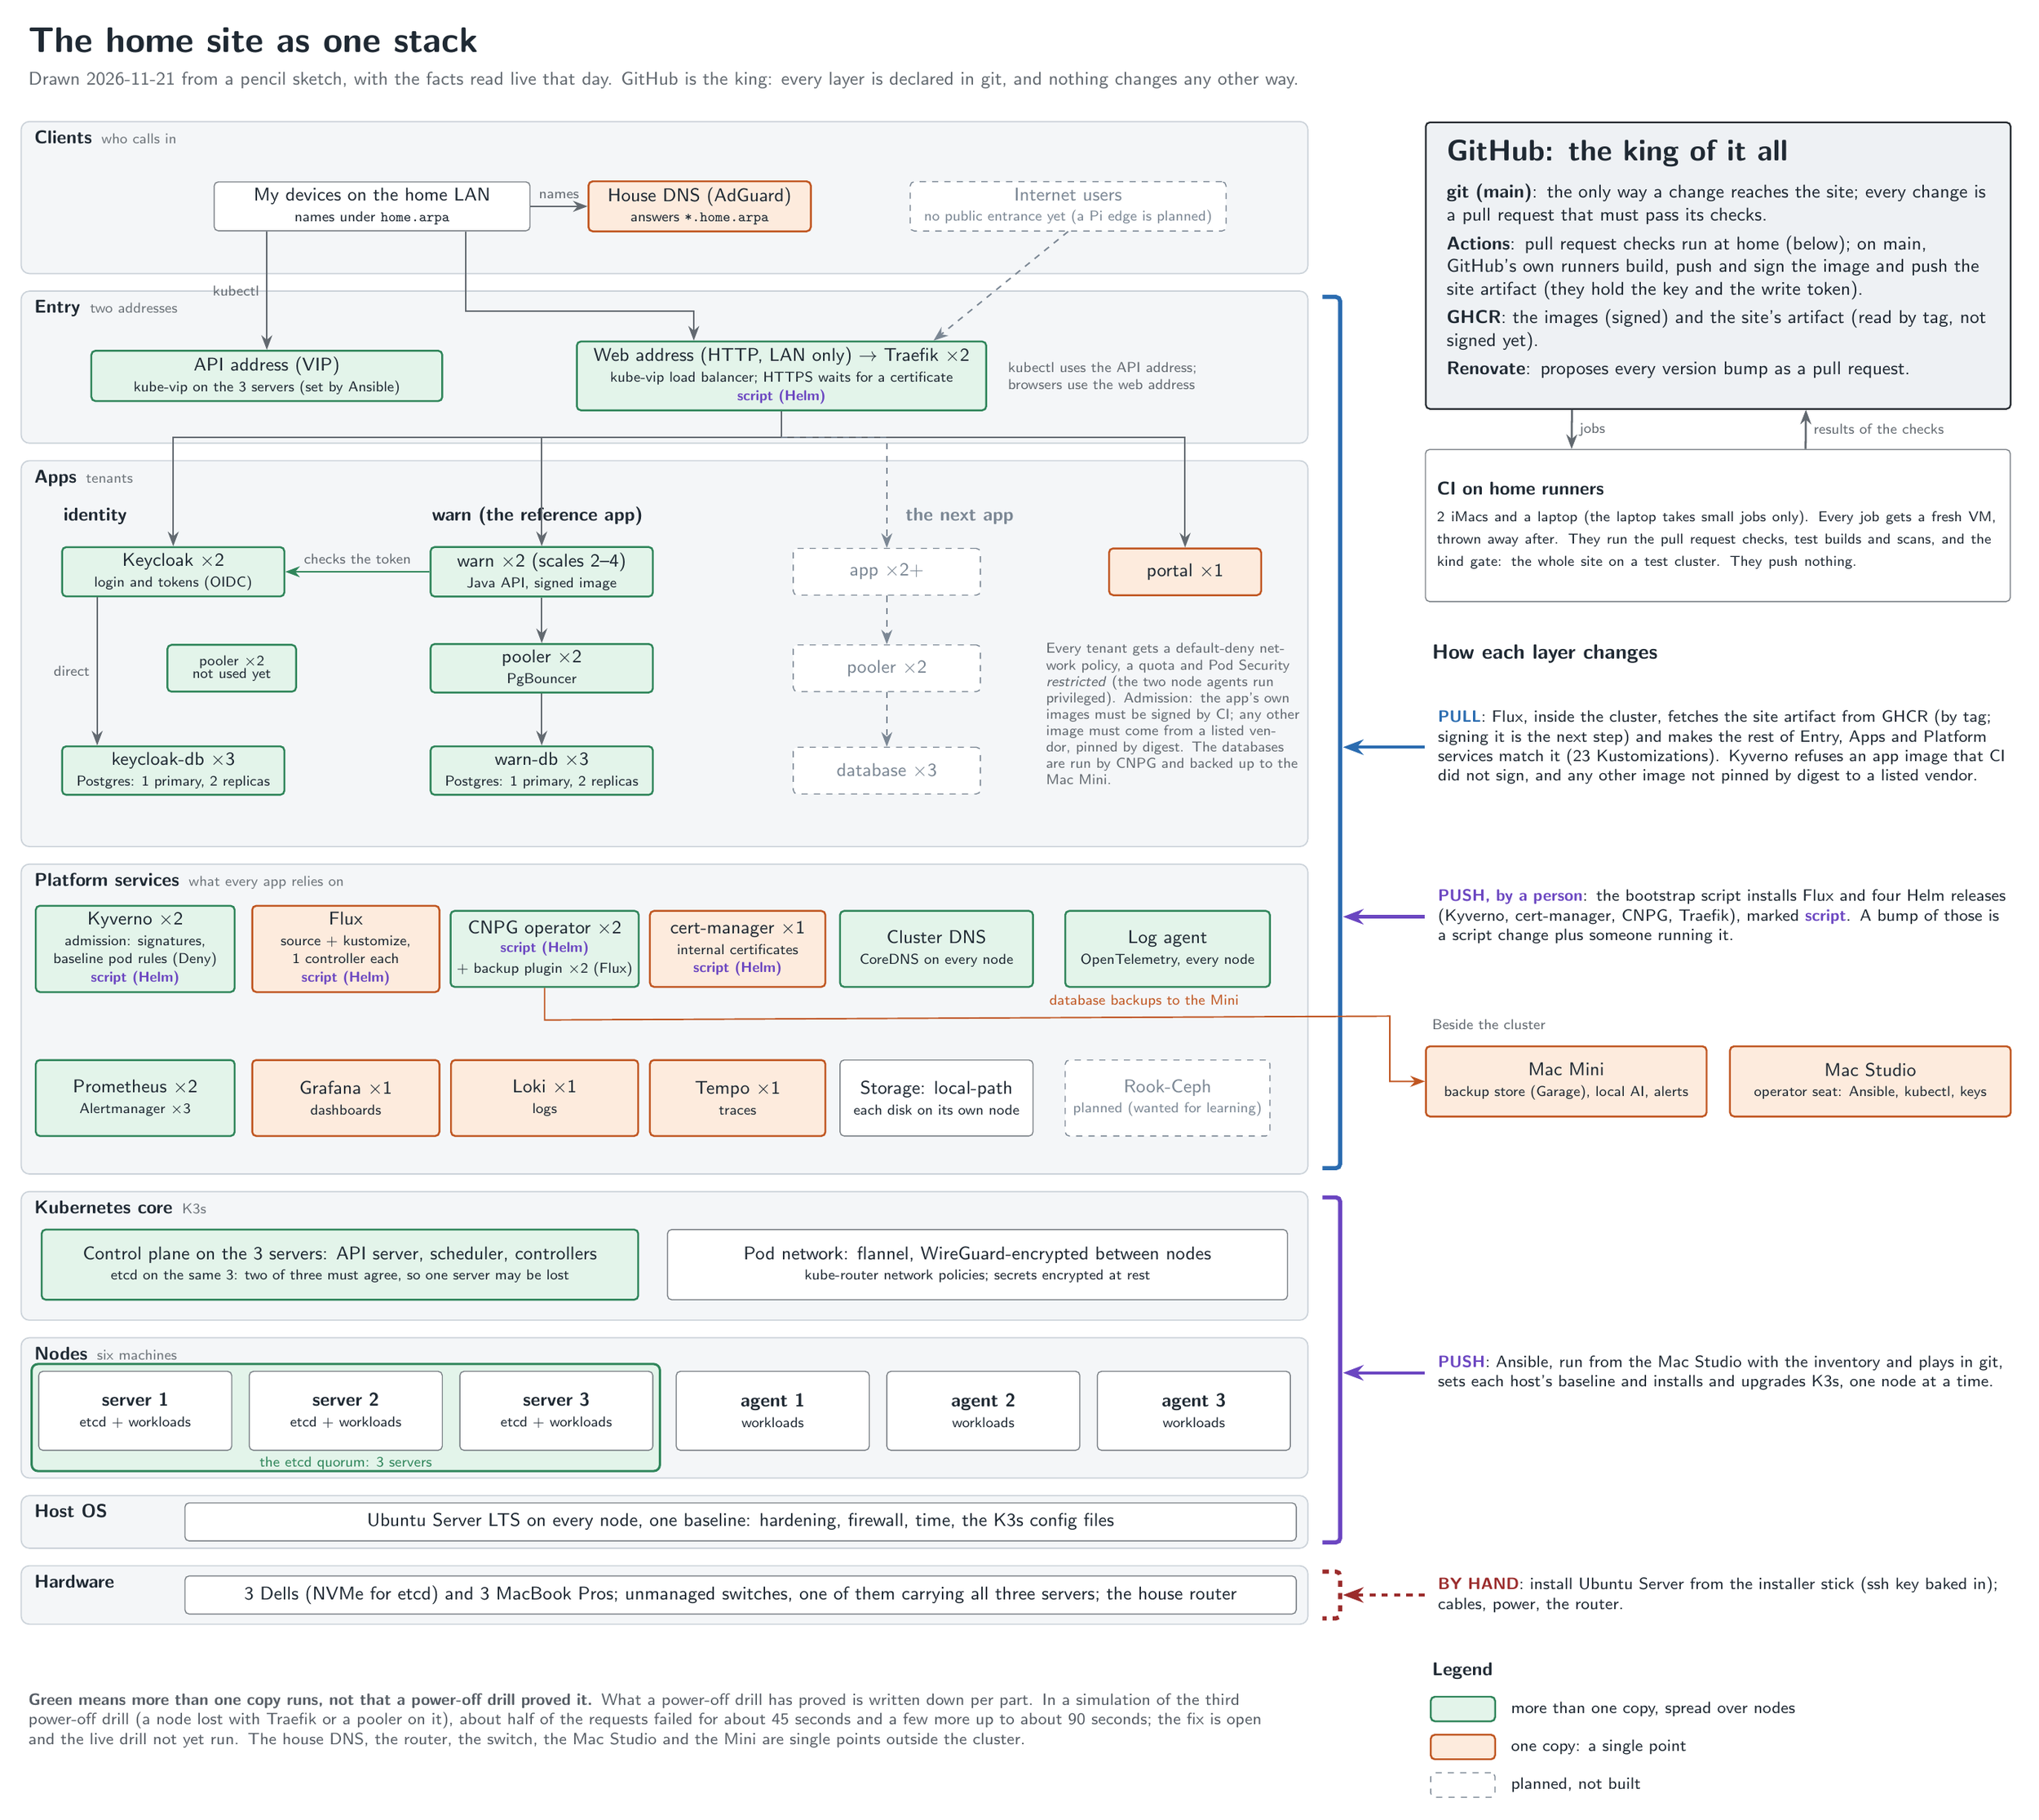
\begin{tikzpicture}[x=1cm, y=1cm]

% ---------------------------------------------------------------- title
\node[anchor=west, font=\bfseries\LARGE] at (0, 27.4) {The home site as one stack};
\node[anchor=west, font=\small, text=ink!70] at (0, 26.7)
  {Drawn 2026-11-21 from a pencil sketch, with the facts read live that day. GitHub is the king: every layer is declared in git, and nothing changes any other way.};

% ---------------------------------------------------------------- layer bands (x 0..22)
\newcommand{\band}[4]{% y-bottom, y-top, name, what
  \draw[layer] (0,#1) rectangle (22,#2);
  \node[anchor=north west, inner sep=2pt] at (0.15,#2-0.08) {\textbf{#3}\enspace{\scriptsize\color{ink!65}#4}};}
\band{23.4}{26.0}{Clients}{who calls in}
\band{20.5}{23.1}{Entry}{two addresses}
\band{13.6}{20.2}{Apps}{tenants}
\band{8.0}{13.3}{Platform services}{what every app relies on}
\band{5.5}{7.7}{Kubernetes core}{K3s}
\band{2.8}{5.2}{Nodes}{six machines}
\band{1.6}{2.5}{Host OS}{}
\band{0.3}{1.3}{Hardware}{}

% ---------------------------------------------------------------- clients
\node[box, minimum width=5.4cm] (owner) at (6.0,24.55) {My devices on the home LAN\\[-1pt]\scriptsize names under \texttt{home.arpa}};
\node[single, minimum width=3.8cm] (housedns) at (11.6,24.55) {House DNS (AdGuard)\\[-1pt]\scriptsize answers \texttt{*.home.arpa}};
\node[plan, minimum width=5.4cm] (internet) at (17.9,24.55) {Internet users\\[-1pt]\scriptsize no public entrance yet (a Pi edge is planned)};
\draw[flow] (owner.east) -- node[above, tag] {names} (housedns.west);

% ---------------------------------------------------------------- entry
\node[multi, minimum width=6.0cm] (apivip) at (4.2,21.65) {API address (VIP)\\[-1pt]\scriptsize kube-vip on the 3 servers (set by Ansible)};
\node[multi, minimum width=7.0cm] (webip) at (13.0,21.65) {Web address (HTTP, LAN only) $\to$ Traefik $\times$2\\[-1pt]\scriptsize kube-vip load balancer; HTTPS waits for a certificate\script};
\node[tag, align=left, anchor=west] at (16.75,21.65) {kubectl uses the API address;\\browsers use the web address};
\draw[flow] ($(owner.south)+(-1.8,0)$) -- node[left, tag] {kubectl} ($(apivip.north)+(0,0)$ -| {$(owner.south)+(-1.8,0)$});
\draw[flow] ($(owner.south)+(1.6,0)$) |- ($(webip.north)+(-1.5,0.5)$) -- ($(webip.north)+(-1.5,0)$);
\draw[flow, dashed, draw=plan] (internet.south) -- ($(webip.north)+(2.6,0)$);

% ---------------------------------------------------------------- apps
\node[font=\bfseries\small, anchor=west] at (0.6,19.25) {identity};
\node[multi, minimum width=3.8cm] (kc) at (2.6,18.3) {Keycloak $\times$2\\[-1pt]\scriptsize login and tokens (OIDC)};
\node[multi, minimum width=2.2cm, font=\scriptsize] (kcpool) at (3.6,16.65) {pooler $\times$2\\[-2pt]not used yet};
\node[multi, minimum width=3.8cm] (kcdb) at (2.6,14.9) {keycloak-db $\times$3\\[-1pt]\scriptsize Postgres: 1 primary, 2 replicas};
\draw[flow] ($(kc.south)+(-1.3,0)$) -- node[left, tag] {direct} ($(kcdb.north)+(-1.3,0)$);

\node[font=\bfseries\small, anchor=west] at (6.9,19.25) {warn (the reference app)};
\node[multi, minimum width=3.8cm] (warn) at (8.9,18.3) {warn $\times$2 (scales 2--4)\\[-1pt]\scriptsize Java API, signed image};
\node[multi, minimum width=3.8cm] (warnpool) at (8.9,16.65) {pooler $\times$2\\[-1pt]\scriptsize PgBouncer};
\node[multi, minimum width=3.8cm] (warndb) at (8.9,14.9) {warn-db $\times$3\\[-1pt]\scriptsize Postgres: 1 primary, 2 replicas};
\draw[flow] (warn) -- (warnpool);
\draw[flow] (warnpool) -- (warndb);
\draw[flow, draw=multi] (warn.west) -- node[above, tag] {checks the token} (kc.east);

\node[font=\bfseries\small, anchor=west, text=plan] at (15.0,19.25) {the next app};
\node[plan, minimum width=3.2cm] (xapp) at (14.8,18.3) {app $\times$2+};
\node[plan, minimum width=3.2cm] (xpool) at (14.8,16.65) {pooler $\times$2};
\node[plan, minimum width=3.2cm] (xdb) at (14.8,14.9) {database $\times$3};
\draw[flow, draw=plan, dashed] (xapp) -- (xpool);
\draw[flow, draw=plan, dashed] (xpool) -- (xdb);

\node[single, minimum width=2.6cm] (portal) at (19.9,18.3) {portal $\times$1};
\node[tag, align=left, anchor=north west, text width=4.4cm] at (17.4,17.2)
  {Every tenant gets a default-deny network policy, a quota and Pod Security \emph{restricted} (the two node agents run privileged). Admission: the app's own images must be signed by CI; any other image must come from a listed vendor, pinned by digest. The databases are run by CNPG and backed up to the Mac Mini.};

% traffic from the web address to the apps
\coordinate (fan) at ($(webip.south)+(0,-0.45)$);
\draw[line width=0.7pt, draw=ink!70] (webip.south) -- (fan);
\draw[flow] (fan) -| (kc.north);
\draw[flow] (fan) -| (warn.north);
\draw[flow] (fan) -| (portal.north);
\draw[flow, dashed, draw=plan] (fan) -| (xapp.north);

% ---------------------------------------------------------------- platform services
\newcommand{\svc}[5]{\node[#1, minimum width=#2, minimum height=1.3cm] (#3) at #4 {#5};}
\svc{multi}{3.4cm}{kyverno}{(1.95,11.85)}{Kyverno $\times$2\\[-1pt]\scriptsize admission: signatures,\\[-2pt]\scriptsize baseline pod rules (Deny)\script}
\svc{single}{3.2cm}{flux}{(5.55,11.85)}{Flux\\[-1pt]\scriptsize source + kustomize,\\[-2pt]\scriptsize 1 controller each\script}
\svc{multi}{3.2cm}{cnpg}{(8.95,11.85)}{CNPG operator $\times$2\script\\[-1pt]\scriptsize + backup plugin $\times$2 (Flux)}
\svc{single}{3.0cm}{certm}{(12.25,11.85)}{cert-manager $\times$1\\[-1pt]\scriptsize internal certificates\script}
\svc{multi}{3.3cm}{dns}{(15.65,11.85)}{Cluster DNS\\[-1pt]\scriptsize CoreDNS on every node}
\svc{multi}{3.5cm}{logagent}{(19.6,11.85)}{Log agent\\[-1pt]\scriptsize OpenTelemetry, every node}
\svc{multi}{3.4cm}{prom}{(1.95,9.3)}{Prometheus $\times$2\\[-1pt]\scriptsize Alertmanager $\times$3}
\svc{single}{3.2cm}{graf}{(5.55,9.3)}{Grafana $\times$1\\[-1pt]\scriptsize dashboards}
\svc{single}{3.2cm}{loki}{(8.95,9.3)}{Loki $\times$1\\[-1pt]\scriptsize logs}
\svc{single}{3.0cm}{tempo}{(12.25,9.3)}{Tempo $\times$1\\[-1pt]\scriptsize traces}
\svc{box}{3.3cm}{storage}{(15.65,9.3)}{Storage: local-path\\[-1pt]\scriptsize each disk on its own node}
\svc{plan}{3.5cm}{ceph}{(19.6,9.3)}{Rook-Ceph\\[-1pt]\scriptsize planned (wanted for learning)}

% ---------------------------------------------------------------- kubernetes core
\node[multi, minimum width=10.2cm, minimum height=1.2cm] (cp) at (5.45,6.45)
  {Control plane on the 3 servers: API server, scheduler, controllers\\[-1pt]\scriptsize etcd on the same 3: two of three must agree, so one server may be lost};
\node[box, minimum width=10.6cm, minimum height=1.2cm] (net) at (16.35,6.45)
  {Pod network: flannel, WireGuard-encrypted between nodes\\[-1pt]\scriptsize kube-router network policies; secrets encrypted at rest};

% ---------------------------------------------------------------- nodes
\draw[multi, line width=1.1pt, rounded corners=3pt, fill=multifill]
  (0.18,4.75) rectangle (10.92,2.92);
\newcommand{\nodebox}[3]{\node[box, minimum width=3.3cm, minimum height=1.35cm] (#1) at #2 {#3};}
\nodebox{s1}{(1.95,3.95)}{\textbf{server 1}\\[-1pt]\scriptsize etcd + workloads}
\nodebox{s2}{(5.55,3.95)}{\textbf{server 2}\\[-1pt]\scriptsize etcd + workloads}
\nodebox{s3}{(9.15,3.95)}{\textbf{server 3}\\[-1pt]\scriptsize etcd + workloads}
\nodebox{a1}{(12.85,3.95)}{\textbf{agent 1}\\[-1pt]\scriptsize workloads}
\nodebox{a2}{(16.45,3.95)}{\textbf{agent 2}\\[-1pt]\scriptsize workloads}
\nodebox{a3}{(20.05,3.95)}{\textbf{agent 3}\\[-1pt]\scriptsize workloads}

\node[tag, text=multi] at (5.55,3.05) {the etcd quorum: 3 servers};

% ---------------------------------------------------------------- host OS and hardware
\node[box, minimum width=19.0cm, minimum height=0.65cm] (os) at (12.3,2.05)
  {Ubuntu Server LTS on every node, one baseline: hardening, firewall, time, the K3s config files};
\node[box, minimum width=19.0cm, minimum height=0.65cm] (hw) at (12.3,0.8)
  {3 Dells (NVMe for etcd) and 3 MacBook Pros; unmanaged switches, one of them carrying all three servers; the house router};

% ================================================================ right side (x 24..34)
\node[ghbox, minimum width=10cm, minimum height=4.9cm, anchor=north west] (gh) at (24.0,26.0) {};
\node[font=\bfseries\Large, anchor=north west] at (24.25,25.8) {GitHub: the king of it all};
\node[anchor=north west, align=left, font=\small, text width=9.4cm] at (24.25,25.05) {%
  \textbf{git (main)}: the only way a change reaches the site; every change is a pull request that must pass its checks.\\[3pt]
  \textbf{Actions}: pull request checks run at home (below); on main, GitHub's own runners build, push and sign the image and push the site artifact (they hold the key and the write token).\\[3pt]
  \textbf{GHCR}: the images (signed) and the site's artifact (read by tag, not signed yet).\\[3pt]
  \textbf{Renovate}: proposes every version bump as a pull request.};

\node[box, minimum width=10cm, minimum height=2.6cm, anchor=north west, align=left, text width=9.6cm] (ci) at (24.0,20.4) {%
  \textbf{CI on home runners}\\[2pt]
  \scriptsize 2 iMacs and a laptop (the laptop takes small jobs only). Every job gets a fresh VM, thrown away after.
  They run the pull request checks, test builds and scans, and the kind gate: the whole site on a test cluster. They push nothing.};
\draw[flow, line width=1pt] ($(gh.south)+(-2.5,0)$) -- node[right, tag] {jobs} ($(ci.north)+(-2.5,0)$);
\draw[flow, line width=1pt] ($(ci.north)+(1.5,0)$) -- node[right, tag] {results of the checks} ($(gh.south)+(1.5,0)$);

\node[font=\bfseries\normalsize, anchor=west] at (24.0,16.9) {How each layer changes};

% PULL: Entry, Apps, Platform services
\draw[bracket, draw=pull] (22.25,23.0) -- (22.55,23.0) -- (22.55,8.1) -- (22.25,8.1);
\draw[-{Stealth[length=3.5mm]}, line width=1.6pt, draw=pull] (24.0,15.3) -- (22.6,15.3);
\node[how, text width=9.8cm] at (24.1,15.3) {\textcolor{pull}{\textbf{PULL}}: Flux, inside the cluster, fetches the site artifact from GHCR (by tag; signing it is the next step) and makes the rest of Entry, Apps and Platform services match it (23 Kustomizations). Kyverno refuses an app image that CI did not sign, and any other image not pinned by digest to a listed vendor.};

% PUSH by script: the four Helm releases
\draw[-{Stealth[length=3.5mm]}, line width=1.6pt, draw=push] (24.0,12.4) -- (22.6,12.4);
\node[how, text width=9.8cm] at (24.1,12.4) {\textcolor{push}{\textbf{PUSH, by a person}}: the bootstrap script installs Flux and four Helm releases (Kyverno, cert-manager, CNPG, Traefik), marked \textcolor{push}{\textbf{script}}. A bump of those is a script change plus someone running it.};

% PUSH by Ansible: core, nodes, host OS
\draw[bracket, draw=push] (22.25,7.6) -- (22.55,7.6) -- (22.55,1.7) -- (22.25,1.7);
\draw[-{Stealth[length=3.5mm]}, line width=1.6pt, draw=push] (24.0,4.6) -- (22.6,4.6);
\node[how, text width=9.8cm] at (24.1,4.6) {\textcolor{push}{\textbf{PUSH}}: Ansible, run from the Mac Studio with the inventory and plays in git, sets each host's baseline and installs and upgrades K3s, one node at a time.};

% BY HAND: hardware and the OS install
\draw[bracket, draw=hand, dashed] (22.25,1.2) -- (22.55,1.2) -- (22.55,0.4) -- (22.25,0.4);
\draw[-{Stealth[length=3.5mm]}, line width=1.6pt, draw=hand, dashed] (24.0,0.8) -- (22.6,0.8);
\node[how, text width=9.8cm] at (24.1,0.8) {\textcolor{hand}{\textbf{BY HAND}}: install Ubuntu Server from the installer stick (ssh key baked in); cables, power, the router.};

% beside the cluster
\node[single, minimum width=4.8cm, minimum height=1.2cm, anchor=north west] (mini) at (24.0,10.2) {Mac Mini\\[-1pt]\scriptsize backup store (Garage), local AI, alerts};
\node[single, minimum width=4.8cm, minimum height=1.2cm, anchor=north west] (studio) at (29.2,10.2) {Mac Studio\\[-1pt]\scriptsize operator seat: Ansible, kubectl, keys};
\node[tag, anchor=west] at (24.0,10.55) {Beside the cluster};
\draw[flow, draw=single] (cnpg.south) -- ++(0,-0.55) -- (23.4,10.7) |- (mini.west) node[pos=0.25, above, tag, sloped] {};
\node[tag, text=single, anchor=south] at (19.2,10.72) {database backups to the Mini};

% ================================================================ legend and note
\node[font=\bfseries\small, anchor=west] at (24.0,-0.5) {Legend};
\node[multi, minimum width=1.1cm, minimum height=0.42cm] at (24.65,-1.15) {};
\node[how] at (25.35,-1.15) {more than one copy, spread over nodes};
\node[single, minimum width=1.1cm, minimum height=0.42cm] at (24.65,-1.8) {};
\node[how] at (25.35,-1.8) {one copy: a single point};
\node[plan, minimum width=1.1cm, minimum height=0.42cm] at (24.65,-2.45) {};
\node[how] at (25.35,-2.45) {planned, not built};
\node[how, text width=21.6cm, text=ink!75] at (0,-1.35) {%
  \textbf{Green means more than one copy runs, not that a power-off drill proved it.} What a power-off drill has proved is
  written down per part. In a simulation of the third power-off drill (a node lost with Traefik or a pooler on it), about half of the requests
  failed for about 45 seconds and a few more up to about 90 seconds; the fix is open and the live drill not yet run. The house DNS, the router, the switch, the Mac Studio and the Mini are single points outside the cluster.};

\end{tikzpicture}
\end{document}
